% 图 22.7 —— 由 `checks/emit_hand.py` 自动拼出（probe 精测 + prims2 图元分解）
%%
% ⚠ 这是**稿子不是成品**：跑 `checks/checkhand.py 22.7` 看指标 + 看叠合图。
%%
%% ⚠ 待核：
%   · 本图 probe 报出阴影族 1 个 —— **本脚本不生成阴影**（要照原书手写）；prims2 的 strokes 里可能含阴影线，核对时留意别画重
%   · 可疑字形 1 项（空心圈 ⊙ 常被认成字母 o）—— 见文件末
%%
\documentclass[12pt]{standalone}
\usepackage{fontspec}
\setsansfont{Arial}
\newfontfamily\mfallback{DejaVu Sans}
\usepackage{tikz}
\begin{document}
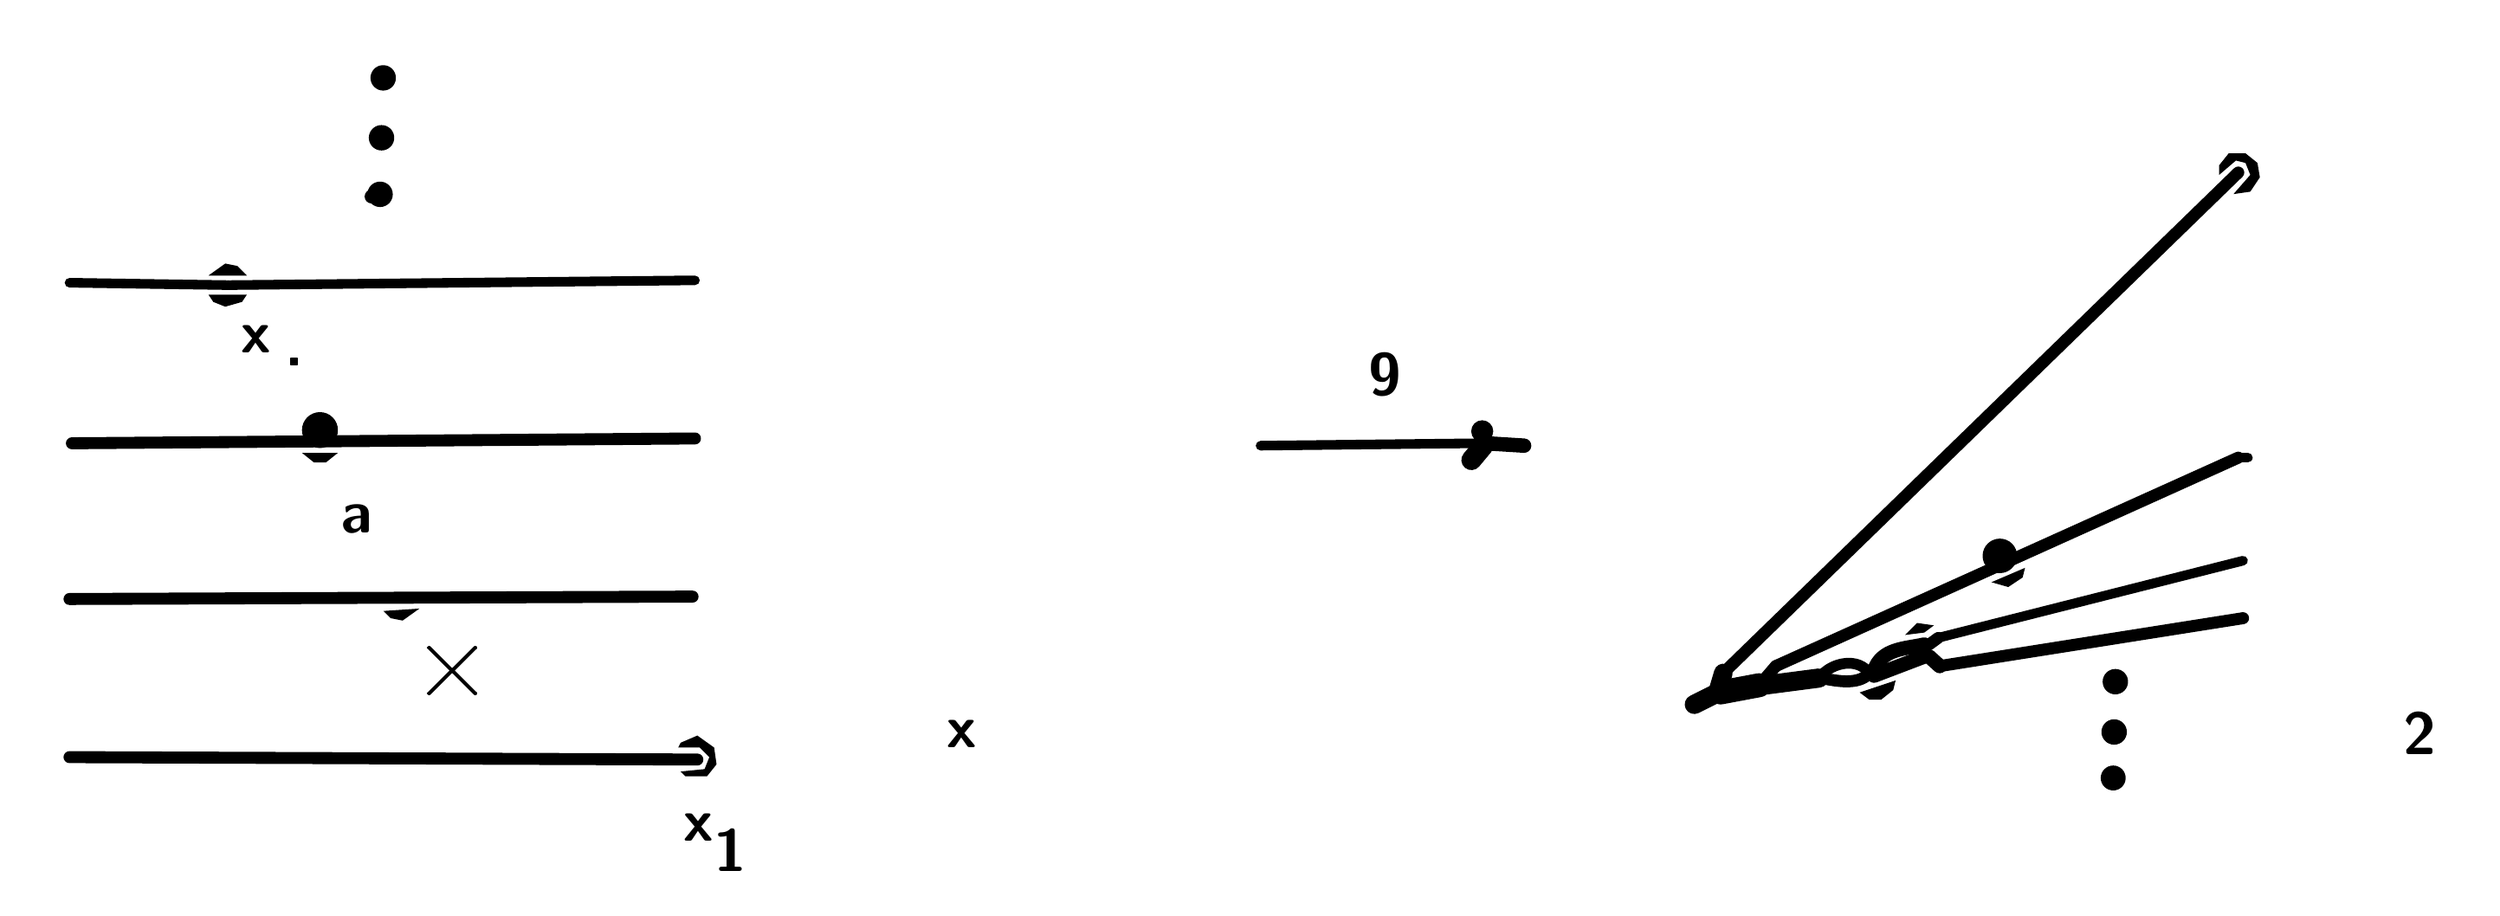
\begin{tikzpicture}[x=1pt, y=-1pt, line width=10.0pt, line cap=round, line join=round]

  %% ════ 填充区（prims2 的 fills）════
  \fill (920.0,54.0) -- (916.0,59.0) -- (916.0,63.0) -- (923.0,57.0) -- (927.0,58.0) -- (929.0,63.0) -- (922.0,71.0) -- (929.0,70.0) -- (933.0,64.0) -- (932.0,58.0) -- (927.0,54.0) -- cycle;
  \fill (77.0,105.0) -- (93.0,105.0) -- (89.0,101.0) -- (84.0,100.0) -- cycle;
  \fill (77.0,113.0) -- (79.0,116.0) -- (84.0,118.0) -- (91.0,116.0) -- (93.0,113.0) -- cycle;
  \fill (116.0,179.0) -- (121.0,183.0) -- (126.0,183.0) -- (131.0,179.0) -- cycle;
  \fill (835.0,227.0) -- (821.0,233.0) -- (828.0,235.0) -- (834.0,231.0) -- cycle;
  \fill (150.0,245.0) -- (153.0,248.0) -- (158.0,249.0) -- (165.0,244.0) -- cycle;
  \fill (785.0,255.0) -- (793.0,254.0) -- (797.0,251.0) -- (790.0,250.0) -- cycle;
  \fill (781.0,274.0) -- (766.0,279.0) -- (770.0,282.0) -- (775.0,282.0) -- (780.0,278.0) -- cycle;
  \fill (274.0,300.0) -- (273.0,302.0) -- (282.0,302.0) -- (286.0,306.0) -- (284.0,311.0) -- (274.0,312.0) -- (276.0,314.0) -- (285.0,314.0) -- (289.0,309.0) -- (288.0,302.0) -- (281.0,297.0) -- cycle;

  %% ════ 直线段（prims2 的 strokes）════
  \draw[line width=10.0pt] (724.0,276.0) -- (708.0,279.0);
  \draw[line width=3.0pt] (794.0,263.0) -- (794.0,260.0);
  \draw[line width=8.4pt] (604.0,182.0) -- (609.0,176.0);
  \draw[line width=6.0pt] (795.0,264.0) -- (799.4,268.0);
  \draw[line width=5.0pt] (799.4,268.0) -- (926.0,248.0);
  \draw[line width=8.0pt] (749.0,273.0) -- (726.0,276.0);
  \draw[line width=5.0pt] (281.0,307.0) -- (19.0,306.0);
  \draw[line width=5.0pt] (725.0,275.0) -- (731.0,268.0);
  \draw[line width=5.0pt] (731.0,268.0) -- (924.0,181.0);
  \draw[line width=4.0pt] (924.0,181.0) -- (928.0,181.0);
  \draw[line width=6.0pt] (772.0,272.0) -- (793.0,264.0);
  \draw[line width=4.0pt] (280.0,107.0) -- (85.2,109.0);
  \draw[line width=4.0pt] (85.2,109.0) -- (19.0,108.0);
  \draw[line width=5.0pt] (280.0,173.0) -- (20.0,175.0);
  \draw[line width=8.0pt] (697.0,284.0) -- (707.0,279.0);
  \draw[line width=6.0pt] (610.0,175.0) -- (626.0,176.0);
  \draw[line width=5.7pt] (145.0,72.0) -- (150.0,72.0);
  \draw[line width=4.0pt] (607.0,175.0) -- (516.0,176.0);
  \draw[line width=5.0pt] (19.0,240.0) -- (279.0,239.0);
  \draw[line width=4.0pt] (926.0,224.0) -- (798.8,256.2);
  \draw[line width=4.9pt] (798.8,256.2) -- (795.0,259.0);
  \draw[line width=7.8pt] (707.0,278.0) -- (709.1,270.9);
  \draw[line width=5.0pt] (709.1,270.9) -- (924.0,62.0);

  %% ════ 曲线（prims2 的 curves —— 三段式，坐标同为 (y,x)）════
  \draw[line width=6.0pt] (772.0,270.0) .. controls (775.0,260.5) and (785.2,260.8) .. (793.0,259.0);
  \draw[line width=4.5pt] (770.0,271.0) .. controls (765.4,264.2) and (754.5,266.5) .. (750.0,272.0);
  \draw[line width=5.0pt] (770.0,271.0) .. controls (765.4,276.2) and (755.9,274.1) .. (750.0,273.0);

  %% ════ 实心点 ════
  \fill (149.9,22.5) circle (5.3);
  \fill (149.2,47.5) circle (5.3);
  \fill (148.6,71.1) circle (5.3);
  \fill (872.7,274.5) circle (5.3);
  \fill (872.2,295.5) circle (5.3);
  \fill (871.8,314.7) circle (5.2);
  \fill (123.5,169.5) circle (7.5);
  \fill (608.5,170.0) circle (4.6);
  \fill (824.5,222.0) circle (7.2);

  %% ════ 标签（probe 直接给的 \node 行）════
  %% ⚠ 全部补了 fill=white：文字在最上层，否则与曲线交叉干扰
     \node[anchor=center,inner sep=0pt,fill=white,font=\fontsize{29.2}{36.5}\selectfont] at (97.0,131.4) {\textsf{\textbf{\textit{x}}}};   % box(88,121,16,17)
     \node[anchor=center,inner sep=0pt,fill=white,font=\fontsize{70.4}{88.0}\selectfont] at (112.8,141.1) {\textsf{\textbf{.}}};   % box(102,132,11,17)
     \node[anchor=center,inner sep=0pt,fill=white,font=\fontsize{34.8}{43.5}\selectfont] at (568.0,146.4) {\textsf{\textbf{9}}};   % box(557,134,18,23)
     \node[anchor=center,inner sep=0pt,fill=white,font=\fontsize{51.3}{64.1}\selectfont] at (139.2,206.6) {\textsf{\textbf{\textit{a}}}};   % box(125,190,25,28)
     \node[anchor=center,inner sep=0pt,fill=white,font=\fontsize{59.9}{74.9}\selectfont] at (179.0,270.0) {\textsf{\textbf{×}}};   % box(165,251,26,29)
     \node[anchor=center,inner sep=0pt,fill=white,font=\fontsize{37.2}{46.5}\selectfont] at (391.2,296.5) {\textsf{\textbf{\textit{x}}}};   % box(380,283,20,22)
     \node[anchor=center,inner sep=0pt,fill=white,font=\fontsize{35.2}{44.0}\selectfont] at (999.9,296.1) {\textsf{\textbf{2}}};   % box(990,284,18,23)
     \node[anchor=center,inner sep=0pt,fill=white,font=\fontsize{30.1}{37.6}\selectfont] at (281.5,335.5) {\textsf{\textbf{\textit{x}}}};   % box(272,325,17,17)
     \node[anchor=center,inner sep=0pt,fill=white,font=\fontsize{23.0}{28.7}\selectfont] at (294.7,344.9) {\textsf{\textbf{1}}};   % box(288,337,8,15)

  % 钉死画布：否则超出的图元/控制点会把页面撑大，1:1 回比就失准
  \pgfresetboundingbox
  \path[use as bounding box] (0,0) rectangle (1023,362);
\end{tikzpicture}
\end{document}

% ⚠ 待核清单（probe 拿不准，人眼过一遍）：
%   · 未识别/跳过：⑤ 跳过/未识别的字形
